%!TeX program = lualatex
\renewcommand{\thelektion}{L09 \textperiodcentered{} Logische Gatter II}
\usetikzlibrary{circuits.logic.US}

\begin{frame}\lessontitle{Lektion 09}{Logische Gatter II}{XOR und Addierer; optional: NAND und funktionale Vollständigkeit \textperiodcentered{} Skript, Kapitel 4}\end{frame}

\begin{frame}\FDUtitle{Rückblick}
\begin{center}
Letztes Mal: NOT, AND, OR -- die drei elementaren Booleschen Verknüpfungen.
\vspace{4mm}

Heute: XOR und Addierer. Optional vertiefen wir NAND als Gatter, aus dem sich \textbf{alle} anderen bauen lassen.
\end{center}
\end{frame}

\begin{frame}\FDUtitle{Optional: Das NAND-Gatter}
\begin{columns}[c,onlytextwidth]
\begin{column}{.46\textwidth}
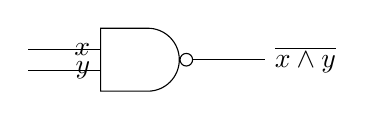
\begin{tikzpicture}[circuit logic US, scale=1.3]
    \node[nand gate, draw] (nand1) {};
    \draw (nand1.input 1) ++(-0.7,0) -- (nand1.input 1) node[left] {$x$};
    \draw (nand1.input 2) ++(-0.7,0) -- (nand1.input 2) node[left] {$y$};
    \draw (nand1.output) -- ++(0.7,0) node[right] {$\overline{x \wedge y}$};
\end{tikzpicture}

\end{column}
\begin{column}{.46\textwidth}
\begin{tabular}{ccc}
    $x$ & $y$ & $\overline{x \wedge y}$ \\\midrule
    0 & 0 & 1 \\
    0 & 1 & 1 \\
    1 & 0 & 1 \\
    1 & 1 & 0 \\
\end{tabular}
\end{column}
\end{columns}
\vspace{3mm}
\begin{center}$\overline{x \wedge y}$ -- die Negation von AND (NOT-AND).\end{center}
\end{frame}

\begin{frame}\FDUtitle{Optional: Funktional vollständig}
\begin{center}
Aus Kombinationen von NAND-Gattern lassen sich \textbf{alle} anderen logischen Funktionen nachbauen.
\vspace{4mm}

\textbf{Challenge (optional)}: Stellen Sie die Wahrheitstabelle von $\overline{x \wedge x}$ auf. Was fällt auf?
\end{center}
\only<2->{
\begin{center}
\begin{tabular}{ccc}
    $x$ & $x \wedge x$ & $\overline{x \wedge x}$ \\\midrule
    0 & 0 & 1 \\
    1 & 1 & 0 \\
\end{tabular}
\end{center}
\begin{center}\color{FDUteal}\bfseries $\overline{x \wedge x} = \overline{x}$ -- ein NOT-Gatter aus einem einzigen NAND!\end{center}
}
\end{frame}

\begin{frame}\FDUtitle{Optional: Warum ist NAND relevant?}
\begin{itemize}
    \item \textbf{Theorie \& Didaktik:} NAND ist ein \enquote{Universalbaustein} (funktionale Vollständigkeit) -- jeder beliebige Computer lässt sich im Prinzip rein aus NAND-Gattern aufbauen.
    \item \textbf{Historisch:} Der \textit{Apollo Guidance Computer} (1966) bestand fast ausschliesslich aus einheitlichen NOR-Gattern zur Fehlerminimierung.
    \item \textbf{Moderne Chips:} Nutzen optimierte Standard-Zellbibliotheken mit massgeschneiderten Transistorlayouts pro Gattertyp (für maximale Geschwindigkeit und minimale Fläche).
\end{itemize}
\end{frame}

\begin{frame}\FDUtitle{Das XOR-Gatter}
\begin{columns}[c,onlytextwidth]
\begin{column}{.46\textwidth}
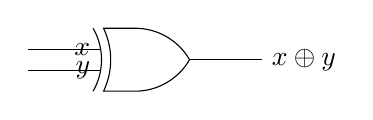
\begin{tikzpicture}[circuit logic US, scale=1.3]
    \node[xor gate, draw] (xor1) {};
    \draw (xor1.input 1) ++(-0.7,0) -- (xor1.input 1) node[left] {$x$};
    \draw (xor1.input 2) ++(-0.7,0) -- (xor1.input 2) node[left] {$y$};
    \draw (xor1.output) -- ++(0.7,0) node[right] {$x \oplus y$};
\end{tikzpicture}

\end{column}
\begin{column}{.46\textwidth}
\begin{tabular}{ccc}
    $x$ & $y$ & $x \oplus y$ \\\midrule
    0 & 0 & 0 \\
    0 & 1 & 1 \\
    1 & 0 & 1 \\
    1 & 1 & 0 \\
\end{tabular}
\end{column}
\end{columns}
\end{frame}

{\setbeamertemplate{footline}{\darkfootline}
\begin{frame}\sectionframe[FDUgreen]{Der Halbaddierer}{Wenn Gatter tatsächlich rechnen}
\end{frame}}

\begin{frame}\FDUtitle{Zwei Bits addieren}
\begin{center}
\begin{tabular}{cc}
    $x$ & $y$ \\\midrule
    0 & 0 \\
    0 & 1 \\
    1 & 0 \\
    1 & 1 \\
\end{tabular}
\quad$\longrightarrow$\quad
\begin{tabular}{cc}
    Übertrag $c$ & Summe $s$ \\\midrule
    0 & 0 \\
    0 & 1 \\
    0 & 1 \\
    1 & 0 \\
\end{tabular}
\end{center}
\begin{center}
Erkennen Sie zwei bekannte Gatter in diesen Spalten?
\end{center}
\only<2->{\begin{center}\color{FDUteal}\bfseries $c = x \wedge y$ (AND), \quad $s = x \oplus y$ (XOR)\end{center}}
\end{frame}

\begin{frame}\FDUtitle{Schaltplan des Halbaddierers}
\begin{center}
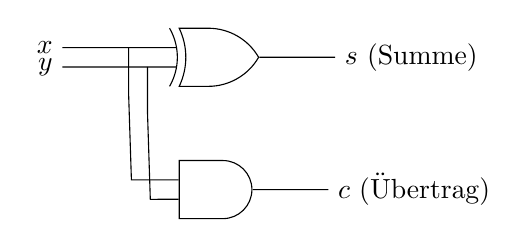
\begin{tikzpicture}[circuit logic US, scale=1.2]
    \begin{scope}[local bounding box=haBB]
        \coordinate (ha-base) at (2,0.5);
        \coordinate (ha-and-pos) at ($(ha-base)+(0,-1.4)$);
        \node[xor gate, draw] (xor1) at (ha-base) {};
        \node[and gate, draw] (and1) at (ha-and-pos) {};

        \coordinate (ha-x-left) at ($(xor1.input 1)+(-1.2,0)$);
        \coordinate (ha-x-split) at ($(xor1.input 1)+(-0.5,0)$);
        \coordinate (ha-x-and) at ($(and1.input 1)+(-0.5,0)$);
        \draw (ha-x-left) -- (ha-x-split) -- (xor1.input 1);
        \draw (ha-x-split) -- ++(0,-0.5) -- (ha-x-and) -- (and1.input 1);
        \node[left] at (ha-x-left) {$x$};

        \coordinate (ha-y-left) at ($(xor1.input 2)+(-1.2,0)$);
        \coordinate (ha-y-split) at ($(xor1.input 2)+(-0.3,0)$);
        \coordinate (ha-y-and) at ($(and1.input 2)+(-0.3,0)$);
        \draw (ha-y-left) -- (ha-y-split) -- (xor1.input 2);
        \draw (ha-y-split) -- ++(0,-0.5) -- (ha-y-and) -- (and1.input 2);
        \node[left] at (ha-y-left) {$y$};

        \coordinate (ha-s-right) at ($(xor1.output)+(0.8,0)$);
        \coordinate (ha-c-right) at ($(and1.output)+(0.8,0)$);
        \draw (xor1.output) -- (ha-s-right) node[right] {$s$ (Summe)};
        \draw (and1.output) -- (ha-c-right) node[right] {$c$ (Übertrag)};
    \end{scope}
\end{tikzpicture}

\end{center}
\begin{center}XOR liefert die Summe, AND den Übertrag.\end{center}
\end{frame}

\begin{frame}\FDUtitle{Übung: Halbaddierer-Wahrheitstabelle}
\begin{center}
\small
\begin{tabular}{cccccc}
    $x$ & $y$ & Summe $s$ ($x \oplus y$) & Übertrag $c$ ($x \land y$) & Binär $(cs)_2$ & Dezimal \\\midrule
    0 & 0 & \only<2->{0} & \only<2->{0} & \only<2->{$00_2$} & \only<2->{0} \\
    0 & 1 & \only<2->{1} & \only<2->{0} & \only<2->{$01_2$} & \only<2->{1} \\
    1 & 0 & \only<2->{1} & \only<2->{0} & \only<2->{$01_2$} & \only<2->{1} \\
    1 & 1 & \only<2->{0} & \only<2->{1} & \only<2->{$10_2$} & \only<2->{2} \\
\end{tabular}
\end{center}
\only<2->{\begin{center}\color{FDUteal}\bfseries Der Halbaddierer berechnet alle 4 Fälle der 1-Bit-Addition exakt korrekt!\end{center}}
\end{frame}

{\setbeamertemplate{footline}{\darkfootline}
\begin{frame}\sectionframe[FDUblue]{Der Volladdierer}{Mehrstellige Zahlen addieren mit Übertrag}
\end{frame}}

\begin{frame}\FDUtitle{Warum reicht ein Halbaddierer nicht aus?}
Beim schriftlichen Addieren mehrerer Stellen entsteht aus der vorherigen Stelle ein \textbf{eingehender Übertrag $c_{\text{in}}$}.
\vspace{3mm}
\begin{center}
Ein \textbf{Volladdierer (Full Adder)} verarbeitet \textbf{3 Eingänge}: $x, y$ und $c_{\text{in}}$.
\end{center}
\end{frame}

\begin{frame}\FDUtitle{Aufbau des Volladdierers}
Ein Volladdierer besteht aus \textbf{zwei Halbaddierern} und einem \textbf{OR-Gatter}:
\vspace{3mm}
\begin{center}
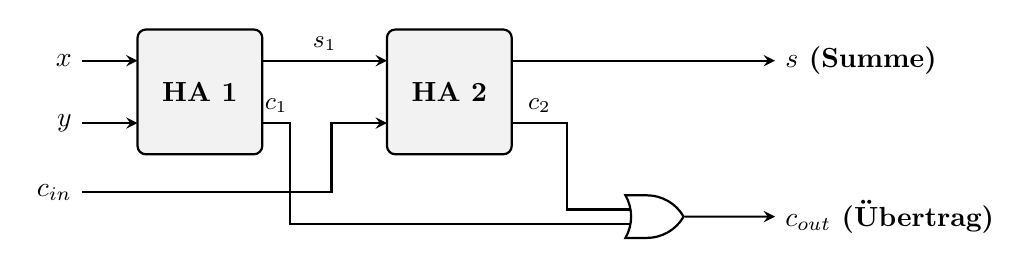
\begin{tikzpicture}[circuit logic US, scale=0.88, >=stealth]
    % Block 1: HA1
    \draw[thick, fill=gray!10, rounded corners=3pt] (0, 0) rectangle (1.8, 1.8);
    \node[font=\normalsize\bfseries] at (0.9, 0.9) {HA 1};
    
    % Block 2: HA2
    \draw[thick, fill=gray!10, rounded corners=3pt] (3.6, 0) rectangle (5.4, 1.8);
    \node[font=\normalsize\bfseries] at (4.5, 0.9) {HA 2};
    
    % OR Gate
    \node[or gate, draw, thick, fill=white] (or1) at (7.4, -0.9) {};

    % Inputs to HA 1
    \draw[thick, ->] (-0.8, 1.35) node[left] {$x$} -- (0, 1.35);
    \draw[thick, ->] (-0.8, 0.45) node[left] {$y$} -- (0, 0.45);
    
    % Sum line from HA 1 to HA 2
    \draw[thick, ->] (1.8, 1.35) -- node[above, font=\small] {$s_1$} (3.6, 1.35);
    
    % Carry-in line to HA 2
    \draw[thick, ->] (-0.8, -0.55) node[left] {$c_{\text{in}}$} -- (2.8, -0.55) |- (3.6, 0.45);
    
    % Final Sum line
    \draw[thick, ->] (5.4, 1.35) -- (9.2, 1.35) node[right] {\textbf{$s$ (Summe)}};
    
    % Carry 1 line (from HA 1 to OR gate input 2)
    \draw[thick] (1.8, 0.45) -- node[above, font=\small] {$c_1$} (2.2, 0.45) |- (or1.input 2);
    
    % Carry 2 line (from HA 2 to OR gate input 1)
    \draw[thick] (5.4, 0.45) -- node[above, font=\small] {$c_2$} (6.2, 0.45) |- (or1.input 1);
    
    % Final Carry-out line
    \draw[thick, ->] (or1.output) -- (9.2, -0.9) node[right] {\textbf{$c_{\text{out}}$ (Übertrag)}};
\end{tikzpicture}




\end{center}
\end{frame}

\begin{frame}\FDUtitle{Schriftliche Binäraddition im Addierwerk}
Mehrere Volladdierer werden kaskadiert (\textit{Ripple-Carry-Addierer}), um ganze Binärzahlen stellenweise zu addieren:
\vspace{2mm}
\begin{center}
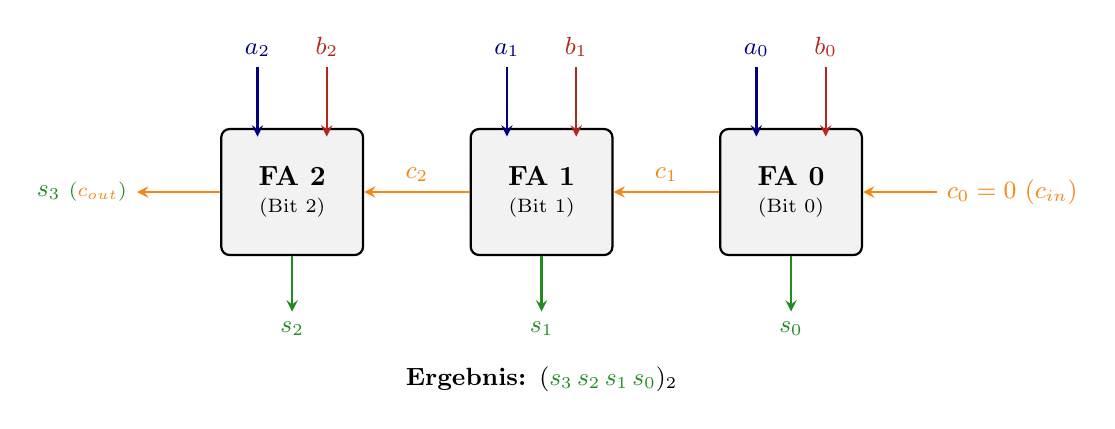
\begin{tikzpicture}[
    scale=0.88, >=stealth,
    fa/.style={draw, thick, fill=gray!10, rounded corners=3pt, minimum width=1.8cm, minimum height=1.6cm, align=center},
    wire/.style={thick, ->}
]
    % FA Blocks (Bit 2 on left, Bit 0 on right)
    \node[fa] (fa2) at (0, 0) {\textbf{FA 2}\\[-2pt]{\scriptsize (Bit 2)}};
    \node[fa] (fa1) at (3.6, 0) {\textbf{FA 1}\\[-2pt]{\scriptsize (Bit 1)}};
    \node[fa] (fa0) at (7.2, 0) {\textbf{FA 0}\\[-2pt]{\scriptsize (Bit 0)}};

    % Inputs from top (a_i in NavyBlue, b_i in BrickRed)
    \draw[wire, NavyBlue] (-0.5, 1.8) node[above, font=\small, NavyBlue] {$a_2$} -- (-0.5, 0.8);
    \draw[wire, BrickRed] (0.5, 1.8) node[above, font=\small, BrickRed] {$b_2$} -- (0.5, 0.8);

    \draw[wire, NavyBlue] (3.1, 1.8) node[above, font=\small, NavyBlue] {$a_1$} -- (3.1, 0.8);
    \draw[wire, BrickRed] (4.1, 1.8) node[above, font=\small, BrickRed] {$b_1$} -- (4.1, 0.8);

    \draw[wire, NavyBlue] (6.7, 1.8) node[above, font=\small, NavyBlue] {$a_0$} -- (6.7, 0.8);
    \draw[wire, BrickRed] (7.7, 1.8) node[above, font=\small, BrickRed] {$b_0$} -- (7.7, 0.8);

    % Carry chain in BurntOrange (from right to left)
    \draw[wire, BurntOrange] (9.3, 0) node[right, font=\small, BurntOrange] {$c_0 = 0$ ($c_{\text{in}}$)} -- (fa0.east);
    \draw[wire, BurntOrange] (fa0.west) -- node[above, font=\small, BurntOrange] {$c_1$} (fa1.east);
    \draw[wire, BurntOrange] (fa1.west) -- node[above, font=\small, BurntOrange] {$c_2$} (fa2.east);
    \draw[wire, BurntOrange] (fa2.west) -- ++(-1.2, 0) node[left, font=\small, ForestGreen] {\textbf{$s_3$} {\scriptsize (\textcolor{BurntOrange}{$c_{\text{out}}$})}};

    % Sum outputs in ForestGreen (to bottom)
    \draw[wire, ForestGreen] (fa2.south) -- ++(0, -0.8) node[below, font=\small, ForestGreen] {\textbf{$s_2$}};
    \draw[wire, ForestGreen] (fa1.south) -- ++(0, -0.8) node[below, font=\small, ForestGreen] {\textbf{$s_1$}};
    \draw[wire, ForestGreen] (fa0.south) -- ++(0, -0.8) node[below, font=\small, ForestGreen] {\textbf{$s_0$}};

    % Summary label
    \node[font=\small\bfseries, align=center] at (3.6, -2.7) {Ergebnis: $(\textcolor{ForestGreen}{s_3 \, s_2 \, s_1 \, s_0})_2$};
\end{tikzpicture}

\end{center}
\begin{center}\color{FDUteal}\bfseries Jede Spalte der Addition wird von genau einem Volladdierer-Baustein berechnet!\end{center}
\end{frame}

\begin{frame}\FDUtitle{Übung: Schriftliche Binäraddition}
\aufgabebox{Berechnen Sie $011_2+010_2$ schriftlich. Beginnen Sie rechts und notieren Sie die Überträge wie bei der Dezimaladdition. Kontrollieren Sie das Ergebnis im Dezimalsystem.}
\vspace{3mm}
\textbf{Hinweis:} Im Binärsystem gilt $1+1=10_2$: Schreiben Sie $0$ und übertragen Sie $1$ in die nächste Spalte.
\end{frame}

\begin{frame}\FDUtitle{Lösung: Schriftliche Binäraddition}
\[
    \begin{array}{rccc}
        & 0 & 1 & 1 \\
        + & 0 & 1 & 0 \\
        \text{Übertrag} & 1 & & \\\hline
        & 1 & 0 & 1
    \end{array}
\]
Von rechts: $1+0=1$; dann $1+1=10_2$, also $0$ schreiben und $1$ übertragen; links $0+0+1=1$. Ergebnis: $101_2=5_{10}$. Kontrolle: $3+2=5$.

\medskip
Jeder Volladdierer übernimmt eine Spalte dieser schriftlichen Rechnung.
\end{frame}

\begin{frame}\FDUtitle{Challenge: Eine Kette von Überträgen}
\challengebox{Berechnen Sie $111_2+001_2$ schriftlich und notieren Sie alle Überträge. Erklären Sie, weshalb links eine zusätzliche Stelle entsteht. Kontrollieren Sie das Ergebnis im Dezimalsystem.}
\end{frame}

\begin{frame}\FDUtitle{Lösung: Eine Kette von Überträgen}
\[
    \begin{array}{rcccc}
        & & 1 & 1 & 1 \\
        + & & 0 & 0 & 1 \\
        \text{Übertrag} & 1 & 1 & 1 & \\\hline
        & 1 & 0 & 0 & 0
    \end{array}
\]
Rechts entsteht durch $1+1=10_2$ ein Übertrag. In den nächsten beiden Spalten ergibt $1+0+1=10_2$ jeweils wieder einen Übertrag. Der letzte Übertrag bildet eine neue linke Stelle. Ergebnis: $1000_2=8_{10}$. Kontrolle: $7+1=8$.
\end{frame}
